\pdfminorversion 7
\pdfobjcompresslevel 3

\documentclass[a4paper]{article}
\special{papersize=210mm,297mm}
\usepackage[utf8]{inputenc}
\usepackage[T1]{fontenc}
\usepackage{cite}
\usepackage[francais]{babel}
\usepackage[bookmarks=false,colorlinks,linkcolor=blue]{hyperref}
\usepackage[top=4cm,bottom=3cm,left=4cm,right=4cm]{geometry}
\usepackage{graphicx}
\usepackage{subfig}
\usepackage{eso-pic}
\usepackage{array}
\usepackage{color}
\usepackage{url}
\usepackage{listings}
\usepackage{eurosym}
\usepackage{url}
\usepackage{textcomp}
\usepackage{fancyhdr} 
\usepackage{tikz}
\usetikzlibrary{automata,positioning}
\usepackage[french]{algorithm2e}

\definecolor{lightgray}{gray}{0.9}

\title{Rapport de projet de PPAR}
\author{Rémy \textsc{El-Sibaie Besognet} -- Roven \textsc{Gabriel}}

\newcommand{\HRule}{\rule{\linewidth}{0.5mm}}


\begin{document}

\maketitle


\section{Introduction}

L'algorithme de Jacobi est une des méthodes de résolution de systèmes
linéaires à diagonales dominantes. C'est le genre de problème qui
fourmille dans l'écosystème de la programmation parallèle de part la
grande quantité de calculs à éffectuer et sa potentielle simplicié à
être exploité par de multiples processeurs.

Le but de ce projet de PPAR est d'analyser une version séquentielle de
la méthode de Jacobi en C, et d'en fournir une version parallèle à
différents niveaux, notemment multi-processus, puis
multi-threading. On utilisera les bibliothèques OpenMPI et OpenMP pour
ce faire. On se posera la question des performancs en fonction des
communications éffectuées et du nombre de processeurs en comparant les
différentes approches. La première, plus naïve, implémentera une
architecture plus simple. On affine cette dernière au fur et à mesure
de l'exercice.

\section{Implémentation} 

\subsection{Condition de terminaison en parallèle}

La méthode de Jacobi correspond à une recherche de point fixe. On
itère jusqu'à ce que le résultat ne change plus. La condition d'arrêt
séquentielle est que la différence entre le résultat de l'itération
précédente et celui de l'opération courante soit inférieure à un
$\epsilon$ petit, c'est à dire la convergence.

Dans le cas parallèle la condition d'arrêt ne change pas, mais elle
doit être calculée sur tous les processus en même temps, c'est quand tous les
processus convergereont que l'ensemble des processus s'arrêteront. Si un
processus fini en avance, il continuera à envoyer les bonnes informations
aux autres sans faire de calcules.

\subsection{Implémentation naïve}

L'approche la plus naïve pour implémenter Jacobi à l'aide de MPI est
d'utiliser une procédure de communication collective
: \texttt{MPI\_Allgather}. Celle-ci est faite pour servir notre
intérêt : réunir en un seul éléments les parties d'un même résultat,
comme indiqué figure~\ref{allgather}. Le but est de découper la
matrice en $P$ (nombre de processus) blocs de lignes et de réunir les
résultats.


\begin{figure}
\centering
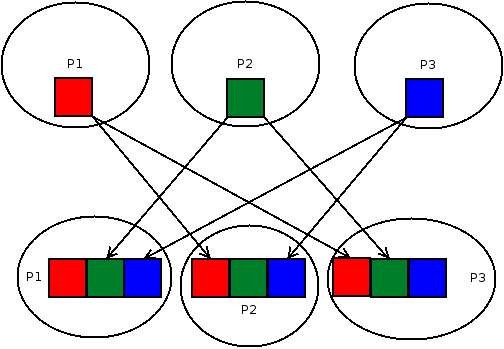
\includegraphics[scale=0.4]{allgather.png}
\caption{\label{allgather}Comportement du MPI\_Allgather}
\end{figure}

On doit s'arranger pour diviser chaque itération sur les différents
processus. La subtilité, dans cette approche est de ne pas oublier la
position de la diagonale dans le bloc de ligne du processus courant.
On admettra simplement, dans chaque processus, que les éléments de la
diagonale ne se trouvent pas en $A[i * h + i] $. Si $hlocal$ est la
hauteur de bloc, on aura une diagonale en $A[i * h + i + hlocal *
rang]$ qui correspond à un décalage de la diagonale de $rang$ fois la
hauteur de bloc.

Étant donné que la convergence de l'ensemble des processus doit être connu
par tous les processus, à chaque itération, un processus donné reçoit une
réduction par l'opérateur de produit des autres convergences. Cette opération
s'éffectue par l'opérateur de communication collective avec 
\texttt{MPI\_Allreduce}.\\

Le pseudo code est détaillé dans l'algorithme~\ref{jacnaif}.

\begin{algorithm}[H]
 \SetLine % For v3.9
 %\SetAlgoLined % For previous releases [?]
 \Repeter{non convergence et iter < maxIter}{
 iter $\leftarrow$ iter + 1\;
 
    \Pour{i = 0 à hlocal}{
     \Pour{j = 0 à n} {
             \dots 
        }
        \dots
      }

    MPI\_Reduce(local\_convergence, convergence, MPI\_PROD)\;
    MPI\_Allgather(xNew, hlocal, xPrev, hlocal)\;

    }
 
 \caption{\label{jacnaif}Jacobi avec \texttt{MPI\_Allgather}}
\end{algorithm}


Cette méthode a l'avantage d'être très simple à la fois à mettre
en \oe uvre et à relire. Mais elle a un énorme problème de
performances. A chaque itération on a $n - 1$ communications par
processus et donc au total une complexité en messages de $n*(n - 1)$,
soit $O(n^2)$. Ceci serait envisageable si il était possible de
recouvrir les communications par du calcul, or ce n'est pas le
cas. C'est pourquoi nous nous tournons vers une autre architecture.

\subsection{Implémentation en anneau}
Une solution possible afin d'éviter l'utilisation des routines de communications 
collectives est d'utiliser une configuration en anneau. Ainsi, au lieu de
reconstruire à chaque itération le \texttt{x-précédent} dans sa globalité, 
chaque processus calculera partiellement son morceau de \texttt{x} en partageant 
sont morceau de \texttt{x-précédent} à la manière d'un \emph{token}. 

A la première itération, un processus calculera son \texttt{x} de départ. Aux
itérations suivantes, le processus calculera partiellement le nouveaux vecteur
\texttt{x} avec le morceau de \texttt{x-précédent} qu'il possède. À la fin de 
ce calcule il enverra ce morceau de \texttt{x-précédent} au processus de rang
$n + 1$ et recevra le morceau de \texttt{x-précédent} du processus de rang
$n - 1$. Lorsqu'un tour complet de l'anneau sera effectué, le calcule des 
\texttt{x} locaux seront terminés, cela marquera la fin d'une itération.

La gestion de l'arrêt est elle aussi gérée sans routine de communication 
collective : à la fin d'une itération, tous les processus envoient 
$convergence~de~gauche~*~convergence$ à leur voisin de droite avec $convergence$
initialisé à leur \emph{convergence locale}. Au bout d'un tour d'anneau, tous
les processus connaitrons l'état global de convergence.\\

Le nombre de messages généré par cette solution est identique à la solution de
communications collectives mais le réseau se trouve moins congestionné ce qui
implique un léger gain de performances globales.

Les points délicats de l'implémentation en anneau se retrouvent dans le 
calcule du \texttt{delta}, le calcul partiel du nouveau \texttt{x} et la colonne
courante. 
\begin{itemize}
\item Dans le calcule du \texttt{delta}, on aura veillé à bien utiliser le 
\texttt{x précédent} du procéssus courant et non le \texttt{x précédent} 
\emph{manipulé} à une itération de l'anneau. 
\item Dans le calcul partiel du nouveau \texttt{x}, on aura veillé à bien utiliser 
la somme partielle précédente plutôt que l'initialiser avec le vecteur \texttt{b}. 

On notera que la division par la diagonale et le calcule de \texttt{delta} ne se 
fait qu'une fois le tour total de l'anneau effectué. 

\item Enfin lors des calcules effectués pendant l'itération sur les 
colonnes de la matrice, il était nécéssaire de considérer un \texttt{j} \emph{réel}
égale à $j~+~source~*~hlocal$ afin de gérer le cas de la diagonale et modifier la 
bonne colonne de la matrice.\\
\end{itemize}

Le pseudo code est détaillé dans l'algorithme~\ref{jacanneau}.

\begin{algorithm}[H]
 \SetLine % For v3.9
 %\SetAlgoLined % For previous releases [?]
 \Repeter{non convergence et iter < maxIter}{
 iter $\leftarrow$ iter + 1\;
 
    \Pour{k = 0 à nombre\_processus}{
      \Pour{i = 0 à hlocal}{
        \Pour{j = 0 à hlocal} {
             \dots 
        }
        \dots
      }
      \dots \\
      MPI\_Sendrecv(xPrev, next\_processus, xPrev, previous\_processus); \\
      \dots
    }

    convergence = convergence\_locale; \\
    \Pour{k = 0 à nombre\_processus}{
      MPI\_Sendrecv(convergence, next\_processus, 
                    convergence\_locale, previous\_processus);\\
      convergence = convergence\_locale * convergence;
    }
  }
 
 \caption{\label{jacanneau}Jacobi avec anneau}
\end{algorithm}

\subsection{Matrice non divisible par $P$}

Dans le cas où la matrice n'est pas divisible par $P$, nous avons fait
le choix d'ajouter au dernier processus les éléments manquant sous
forme de décalage (\emph{offset}). On peut reprendre les algorithmes
décris précédemment en ajoutant le décalage à $hlocal$. Dans le cas de
l'algorithme en anneau, on distingue plusieurs cas :
\begin{itemize}
\item Le processus source courant est le dernier processus : on
considère la largeur du bloc comme étant de $(hlocal + offset)$.
\item Le processus courant est le dernier processus : on considère la
hauteur du bloc comme étant de $(hlocal + offset)$.
\item Les deux assertions précédentes sont vérifiées : on applique les
la modification et la taille du bloc devient : $(hlocal + offset) *
(hlocal + offset)$
\end{itemize}

\subsection{Algorithmes d'initialisation et de vérification}

Les étapes de génération de la matrice, du vecteur et le calcul de du
résidu n'est pas pris en compte dans l'analyse de l'efficacité. Les
algorithmes implémentés sont donc relativement naïfs.

Concernant la matrice, on parallelise simplement la fonction de
génération sans s'occuper du partage ni des communications parce que
la matrice va rester distribuée durant toute l'opération. On utilise
le même algorithme que celui fournit et on créé sur chaque processus
une partie de matrice de taille $hlocal$ dans le cas où la
matrice n'est pas divisible. La génération du vecteur s'inspire
exactement de la même idée, sans subtilité particulière.

Le calcul du résidu est légèrement plus compliqué parce que l'on doit
effectuer une partir du calcul sur chaque processus puis ensuite
réunir ces calculs. Il faut dans un premier temps calculer une partie
du résidu. Pour cela, on parallèlise la boucle de calcul donnée comme
si le vecteur résultat était de taille hlocal. On utilise ensuite une
routine de communication collective. On pourra utiliser MPI\_Gather,
dont le comportement est analogue à MPI\_Allgather sauf qu'il n'y a
qu'un seul processus cible.

\section{Optimisations}

\subsection{Parallèlisation hybride : MPI + OpenMP}
Le calcul du vecteur \texttt{x} est bien découpé sur plusieurs processus possédant
une partie de la matrice totale. Un axe d'optimisation de ce calcul est la
parallélisation du calcul interne à chaque processus qui parcours les lignes de la
matrice local. Cette parallélisation est possible car le calcul de chaque 
composante du vecteur \texttt{x} est indépendante.

Cette optimisation s'éffectue en rajoutant la directive parallele suivantes : \\
\verb|#pragma omp parallel for default(shared) private(c, d)| au dessus de la
boucle de parcours des lignes de la matrice (\emph{pour i} dans l'algoritme~
\ref{jacanneau}). On notera que les variables \texttt{c} et \texttt{d} sont
propres à chaque itération et sont donc définie comme privés. Le restes des
variables sont partagées.\\

Le gain en performance obtenue par une approche hybride MPI + OpenMP est non
négliable avec un temps d'exécution presque divisé par deux entre l'implémentation
simple et l'implémentation avec OpenMP.

\section{Conclusion}

\end{document}

# Local Variables:
# compile-command: "rubber -d rapport.tex"
# End:
